% Options for packages loaded elsewhere
\PassOptionsToPackage{unicode}{hyperref}
\PassOptionsToPackage{hyphens}{url}
%
\documentclass[
]{ctexart}
\usepackage{amsmath,amssymb}
\usepackage{iftex}
\ifPDFTeX
  \usepackage[T1]{fontenc}
  \usepackage[utf8]{inputenc}
  \usepackage{textcomp} % provide euro and other symbols
\else % if luatex or xetex
  \usepackage{unicode-math} % this also loads fontspec
  \defaultfontfeatures{Scale=MatchLowercase}
  \defaultfontfeatures[\rmfamily]{Ligatures=TeX,Scale=1}
\fi
\usepackage{lmodern}
\ifPDFTeX\else
  % xetex/luatex font selection
\fi
% Use upquote if available, for straight quotes in verbatim environments
\IfFileExists{upquote.sty}{\usepackage{upquote}}{}
\IfFileExists{microtype.sty}{% use microtype if available
  \usepackage[]{microtype}
  \UseMicrotypeSet[protrusion]{basicmath} % disable protrusion for tt fonts
}{}
\makeatletter
\@ifundefined{KOMAClassName}{% if non-KOMA class
  \IfFileExists{parskip.sty}{%
    \usepackage{parskip}
  }{% else
    \setlength{\parindent}{0pt}
    \setlength{\parskip}{6pt plus 2pt minus 1pt}}
}{% if KOMA class
  \KOMAoptions{parskip=half}}
\makeatother
\usepackage{xcolor}
\usepackage{color}
\usepackage{fancyvrb}
\newcommand{\VerbBar}{|}
\newcommand{\VERB}{\Verb[commandchars=\\\{\}]}
\DefineVerbatimEnvironment{Highlighting}{Verbatim}{commandchars=\\\{\}}
% Add ',fontsize=\small' for more characters per line
\usepackage{framed}
\definecolor{shadecolor}{RGB}{248,248,248}
\newenvironment{Shaded}{\begin{snugshade}}{\end{snugshade}}
\newcommand{\AlertTok}[1]{\textcolor[rgb]{0.94,0.16,0.16}{#1}}
\newcommand{\AnnotationTok}[1]{\textcolor[rgb]{0.56,0.35,0.01}{\textbf{\textit{#1}}}}
\newcommand{\AttributeTok}[1]{\textcolor[rgb]{0.13,0.29,0.53}{#1}}
\newcommand{\BaseNTok}[1]{\textcolor[rgb]{0.00,0.00,0.81}{#1}}
\newcommand{\BuiltInTok}[1]{#1}
\newcommand{\CharTok}[1]{\textcolor[rgb]{0.31,0.60,0.02}{#1}}
\newcommand{\CommentTok}[1]{\textcolor[rgb]{0.56,0.35,0.01}{\textit{#1}}}
\newcommand{\CommentVarTok}[1]{\textcolor[rgb]{0.56,0.35,0.01}{\textbf{\textit{#1}}}}
\newcommand{\ConstantTok}[1]{\textcolor[rgb]{0.56,0.35,0.01}{#1}}
\newcommand{\ControlFlowTok}[1]{\textcolor[rgb]{0.13,0.29,0.53}{\textbf{#1}}}
\newcommand{\DataTypeTok}[1]{\textcolor[rgb]{0.13,0.29,0.53}{#1}}
\newcommand{\DecValTok}[1]{\textcolor[rgb]{0.00,0.00,0.81}{#1}}
\newcommand{\DocumentationTok}[1]{\textcolor[rgb]{0.56,0.35,0.01}{\textbf{\textit{#1}}}}
\newcommand{\ErrorTok}[1]{\textcolor[rgb]{0.64,0.00,0.00}{\textbf{#1}}}
\newcommand{\ExtensionTok}[1]{#1}
\newcommand{\FloatTok}[1]{\textcolor[rgb]{0.00,0.00,0.81}{#1}}
\newcommand{\FunctionTok}[1]{\textcolor[rgb]{0.13,0.29,0.53}{\textbf{#1}}}
\newcommand{\ImportTok}[1]{#1}
\newcommand{\InformationTok}[1]{\textcolor[rgb]{0.56,0.35,0.01}{\textbf{\textit{#1}}}}
\newcommand{\KeywordTok}[1]{\textcolor[rgb]{0.13,0.29,0.53}{\textbf{#1}}}
\newcommand{\NormalTok}[1]{#1}
\newcommand{\OperatorTok}[1]{\textcolor[rgb]{0.81,0.36,0.00}{\textbf{#1}}}
\newcommand{\OtherTok}[1]{\textcolor[rgb]{0.56,0.35,0.01}{#1}}
\newcommand{\PreprocessorTok}[1]{\textcolor[rgb]{0.56,0.35,0.01}{\textit{#1}}}
\newcommand{\RegionMarkerTok}[1]{#1}
\newcommand{\SpecialCharTok}[1]{\textcolor[rgb]{0.81,0.36,0.00}{\textbf{#1}}}
\newcommand{\SpecialStringTok}[1]{\textcolor[rgb]{0.31,0.60,0.02}{#1}}
\newcommand{\StringTok}[1]{\textcolor[rgb]{0.31,0.60,0.02}{#1}}
\newcommand{\VariableTok}[1]{\textcolor[rgb]{0.00,0.00,0.00}{#1}}
\newcommand{\VerbatimStringTok}[1]{\textcolor[rgb]{0.31,0.60,0.02}{#1}}
\newcommand{\WarningTok}[1]{\textcolor[rgb]{0.56,0.35,0.01}{\textbf{\textit{#1}}}}
\usepackage{graphicx}
\makeatletter
\def\maxwidth{\ifdim\Gin@nat@width>\linewidth\linewidth\else\Gin@nat@width\fi}
\def\maxheight{\ifdim\Gin@nat@height>\textheight\textheight\else\Gin@nat@height\fi}
\makeatother
% Scale images if necessary, so that they will not overflow the page
% margins by default, and it is still possible to overwrite the defaults
% using explicit options in \includegraphics[width, height, ...]{}
\setkeys{Gin}{width=\maxwidth,height=\maxheight,keepaspectratio}
% Set default figure placement to htbp
\makeatletter
\def\fps@figure{htbp}
\makeatother
\setlength{\emergencystretch}{3em} % prevent overfull lines
\providecommand{\tightlist}{%
  \setlength{\itemsep}{0pt}\setlength{\parskip}{0pt}}
\setcounter{secnumdepth}{5}
\usepackage{titling}
\pretitle{\begin{center} 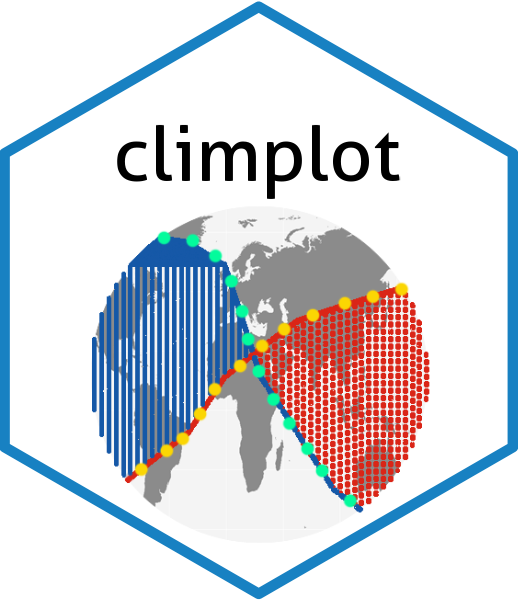
\includegraphics[width=2in,height=2in]{imgfile.png}\LARGE\\}
\posttitle{\end{center}}
\usepackage{booktabs}
\usepackage{longtable}
\usepackage{array}
\usepackage{multirow}
\usepackage{wrapfig}
\usepackage{float}
\usepackage{colortbl}
\usepackage{pdflscape}
\usepackage{tabu}
\usepackage{threeparttable}
\usepackage{threeparttablex}
\usepackage[normalem]{ulem}
\usepackage{makecell}
\usepackage{xcolor}
\ifLuaTeX
  \usepackage{selnolig}  % disable illegal ligatures
\fi
\IfFileExists{bookmark.sty}{\usepackage{bookmark}}{\usepackage{hyperref}}
\IfFileExists{xurl.sty}{\usepackage{xurl}}{} % add URL line breaks if available
\urlstyle{same}
\hypersetup{
  pdftitle={climplot:用于绘制Walter \& Lieth气候图的流程化工具},
  pdfauthor={陈子豪; 在读博士生},
  hidelinks,
  pdfcreator={LaTeX via pandoc}}

\title{climplot:用于绘制Walter \& Lieth气候图的流程化工具}
\author{陈子豪 \and 在读博士生}
\date{}

\begin{document}
\maketitle

{
\setcounter{tocdepth}{2}
\tableofcontents
}
\hypertarget{ux7b80ux4ecb}{%
\section{简介}\label{ux7b80ux4ecb}}

\href{https://gitee.com/auman-chan/climplot}{climplot}
为一个绘图软件包,旨在以更加用户友好和个性化的方式收集全球各地的关键气候数据,并绘制Walter&Lieth气候图。

该软件包的主要作用为:

\begin{itemize}
\item
  使用Worldclim的气候数据来获得标准化和可靠的数据,以构建 Walter&Lieth
  气候图
\item
  提供更多参数定制图片样式和信息显示方式
\end{itemize}

该包提供以下函数功能:

\begin{itemize}
\item
  获取气候数据以构建Walter&Lieth气候图
\item
  绘制Walter&Lieth气候图
\item
  修改气候图的配色和显示的相关信息
\end{itemize}

\hypertarget{ux5b89ux88c5ux4e0eux52a0ux8f7d}{%
\section{安装与加载}\label{ux5b89ux88c5ux4e0eux52a0ux8f7d}}

从\href{https://gitee.com}{gitee}和\href{https://github.com/}{github}
安装最新的开发版本,请安装R包\href{https://cran.r-project.org/package=remotes}{remotes}和\href{https://cran.r-project.org/package=git2r}{git2r}:

\begin{Shaded}
\begin{Highlighting}[]
\FunctionTok{install.packages}\NormalTok{(}\StringTok{\textquotesingle{}remotes\textquotesingle{}}\NormalTok{)}

\CommentTok{\#from github}
\NormalTok{remotes}\SpecialCharTok{::}\FunctionTok{install\_github}\NormalTok{(}\StringTok{"auman{-}chan/climplot"}\NormalTok{)}
\CommentTok{\#from gitee}
\FunctionTok{install.packages}\NormalTok{(}\StringTok{\textquotesingle{}git2r\textquotesingle{}}\NormalTok{)}
\NormalTok{remotes}\SpecialCharTok{::}\FunctionTok{install\_git}\NormalTok{(}\StringTok{"https://gitee.com/auman{-}chan/climplot.git"}\NormalTok{)}
\end{Highlighting}
\end{Shaded}

\hypertarget{ux7ed8ux56feux6570ux636eux63d0ux53d6}{%
\section{绘图数据提取}\label{ux7ed8ux56feux6570ux636eux63d0ux53d6}}

搜索和处理多个地点的气候数据是一项具有挑战性的工作。函数
\texttt{clim\_extract}可以检索来自Worldclim
的历史月度天气数据(2010-2019年2.5度分版本,\url{https://worldclim.org/data/monthlywth.html})的数据,为图表可视化做好准备。

\hypertarget{ux6570ux636eux51c6ux5907}{%
\subsection{数据准备}\label{ux6570ux636eux51c6ux5907}}

\hypertarget{ux6c14ux5019ux6570ux636eux4e0bux8f7d}{%
\subsubsection{气候数据下载}\label{ux6c14ux5019ux6570ux636eux4e0bux8f7d}}

Worldclim气候数据是本软件包必不可少的,由于其全球尺度栅格数据的文件较大,软件包中无法容纳需要的气候数据。因此,请在使用前从\href{NULL}{Figshare}获取对应的气候数据集。

此数据集包括4个文件夹,共48个tif文件,其中包括年均最低气温、年均最高气温、年均降水和年极端最低气温。这些数值是根据2010-2019年的月平均值和最小值计算得出的。数据集的结构如下表所示:

\begin{tabular}{rllll}
\toprule
No & 1 & 2 & 3 & 4\\
\midrule
1 & tmax\_01.tif & tmin\_01.tif & prec\_01.tif & extmin\_01.tif\\
2 & tmax\_02.tif & tmin\_02.tif & prec\_02.tif & extmin\_02.tif\\
3 & tmax\_03.tif & tmin\_03.tif & prec\_03.tif & extmin\_03.tif\\
4 & tmax\_04.tif & tmin\_04.tif & prec\_04.tif & extmin\_04.tif\\
5 & tmax\_05.tif & tmin\_05.tif & prec\_05.tif & extmin\_05.tif\\
\addlinespace
6 & tmax\_06.tif & tmin\_06.tif & prec\_06.tif & extmin\_06.tif\\
7 & tmax\_07.tif & tmin\_07.tif & prec\_07.tif & extmin\_07.tif\\
8 & tmax\_08.tif & tmin\_08.tif & prec\_08.tif & extmin\_08.tif\\
9 & tmax\_09.tif & tmin\_09.tif & prec\_09.tif & extmin\_09.tif\\
10 & tmax\_10.tif & tmin\_10.tif & prec\_10.tif & extmin\_10.tif\\
\addlinespace
11 & tmax\_11.tif & tmin\_11.tif & prec\_11.tif & extmin\_11.tif\\
12 & tmax\_12.tif & tmin\_12.tif & prec\_12.tif & extmin\_12.tif\\
\bottomrule
\multicolumn{5}{l}{\rule{0pt}{1em}\textit{Note: }}\\
\multicolumn{5}{l}{\rule{0pt}{1em}1. 年均最高气温}\\
\multicolumn{5}{l}{\rule{0pt}{1em}2. 年均最低气温}\\
\multicolumn{5}{l}{\rule{0pt}{1em}3. 年均降水}\\
\multicolumn{5}{l}{\rule{0pt}{1em}4. 年极端最低气温}\\
\end{tabular}

\hypertarget{ux76eeux6807ux5730ux70b9ux7684ux4fe1ux606fux51c6ux5907}{%
\subsubsection{目标地点的信息准备}\label{ux76eeux6807ux5730ux70b9ux7684ux4fe1ux606fux51c6ux5907}}

为了提取特定地点的气候数据,精确的坐标是必不可少的。此外,图表应该显示其他相关信息,如位置名称和高度。因此,一个包含目标位置信息的数据框对于clim\_extract来说是必要的。导入的数据框必须包含5列,顺序如下:

\begin{itemize}
\item
  \textbf{No}:目标地点的序号
\item
  \textbf{location}:目标地点的缩写
\item
  \textbf{lon}:目标地点的经度,以十进制表示,负数表示西经
\item
  \textbf{lat}:目标地点的纬度,以十进制表示,负数表示南纬
\item
  \textbf{altitude}:目标地点的高度
\end{itemize}

这个包中的数据 \texttt{locdata} 是
导入格式的例子。上述列的后面允许添加其他包含信息的列,但在后续处理中将被舍弃。

\begin{table}
\centering
\resizebox{\linewidth}{!}{
\begin{tabular}{rlrrrl}
\toprule
No & location & lon & lat & altitude & name\\
\midrule
1 & Motuo & 95.3536 & 29.30420 & 2025 & 墨脱县仁钦崩寺\\
2 & Wulianshan & 100.5000 & 24.50000 & 1301 & 无量山自然保护区\\
3 & Wawushan & 102.9167 & 29.50000 & 2082 & 四川省眉山市洪雅县瓦屋山\\
4 & Leibo & 103.4667 & 28.45000 & 1204 & 四川省凉山州雷波县\\
5 & Longcanggou & 102.8333 & 29.61667 & 1764 & 四川省雅安市荥经县龙苍沟国家森林公园\\
\addlinespace
6 & Jinfoshan & 107.1933 & 29.00017 & 1917 & 重庆市南川区金佛山国家级自然保护区\\
7 & Xishui & 106.4667 & 28.30000 & 863 & 贵州省习水良村镇羊化村\\
8 & Tonglingshan & 119.8598 & 27.82128 & 724 & 浙江省铜铃山国家森林公园\\
9 & Qinglongshan & 112.5341 & 23.17020 & 320 & 广东省鼎湖山自然保护区的百丈岭、青龙山\\
10 & Tiantongshan & 121.7855 & 29.80710 & 199 & 浙江省天童山\\
\bottomrule
\end{tabular}}
\end{table}

\hypertarget{ux6c14ux5019ux6570ux636eux63d0ux53d6}{%
\subsubsection{气候数据提取}\label{ux6c14ux5019ux6570ux636eux63d0ux53d6}}

在准备好气候数据集和位置信息后,导入三个气候数据集的数据框和数据集路径,此函数将导出一个数据框。

\begin{Shaded}
\begin{Highlighting}[]
\CommentTok{\#Modify the path of yours}
\NormalTok{a }\OtherTok{\textless{}{-}} \StringTok{"G:/climplot/climdata/tmin"}
\NormalTok{b }\OtherTok{\textless{}{-}} \StringTok{"G:/climplot/climdata/tmax"}
\NormalTok{c }\OtherTok{\textless{}{-}} \StringTok{"G:/climplot/climdata/prec"}

\CommentTok{\#extraction of climate data}

\NormalTok{plotdata }\OtherTok{\textless{}{-}} \FunctionTok{clim\_extract}\NormalTok{(locdata,a,b,c)}
\ErrorTok{\}}
\end{Highlighting}
\end{Shaded}

\begin{table}
\centering
\resizebox{\linewidth}{!}{
\begin{tabular}{rrlrrlrrrrrrrrrrrr}
\toprule
No & Altitude & Location & Lon & Lat & Type & 1 & 2 & 3 & 4 & 5 & 6 & 7 & 8 & 9 & 10 & 11 & 12\\
\midrule
1 & 2025 & Motuo & 95.3536 & 29.30420 & precipitation & 10.10 & 20.960001 & 44.85 & 98.94 & 136.67 & 232.45 & 243.60 & 204.74 & 207.16 & 74.80 & 9.20 & 5.19\\
1 & 2025 & Motuo & 95.3536 & 29.30420 & min.temprature & -1.10 & 0.600000 & 3.70 & 7.20 & 11.20 & 13.70 & 14.90 & 14.60 & 14.10 & 9.90 & 3.70 & 0.60\\
1 & 2025 & Motuo & 95.3536 & 29.30420 & max.temprature & 12.30 & 13.800000 & 16.50 & 19.20 & 22.70 & 25.10 & 25.50 & 26.10 & 24.00 & 20.80 & 17.60 & 14.10\\
2 & 1301 & Wulianshan & 100.5000 & 24.50000 & precipitation & 17.95 & 7.160000 & 20.38 & 37.63 & 60.43 & 158.30 & 203.94 & 187.86 & 120.89 & 103.53 & 23.70 & 26.15\\
2 & 1301 & Wulianshan & 100.5000 & 24.50000 & min.temprature & 6.80 & 8.500000 & 11.80 & 15.20 & 18.20 & 20.20 & 20.80 & 20.30 & 19.40 & 16.40 & 11.70 & 8.00\\
\addlinespace
2 & 1301 & Wulianshan & 100.5000 & 24.50000 & max.temprature & 21.00 & 24.100000 & 26.70 & 29.00 & 30.10 & 29.00 & 28.40 & 29.00 & 27.80 & 25.30 & 23.30 & 19.90\\
3 & 2082 & Wawushan & 102.9167 & 29.50000 & precipitation & 7.88 & 8.520001 & 24.04 & 59.87 & 100.53 & 195.40 & 180.20 & 164.01 & 163.07 & 62.63 & 15.26 & 11.20\\
3 & 2082 & Wawushan & 102.9167 & 29.50000 & min.temprature & -5.20 & -3.600000 & 0.00 & 4.30 & 7.70 & 10.80 & 13.70 & 13.40 & 10.30 & 5.40 & 1.00 & -3.30\\
3 & 2082 & Wawushan & 102.9167 & 29.50000 & max.temprature & 4.00 & 6.100000 & 10.40 & 14.70 & 17.20 & 18.60 & 21.00 & 21.10 & 16.40 & 12.60 & 9.50 & 5.00\\
4 & 1204 & Leibo & 103.4667 & 28.45000 & precipitation & 9.54 & 9.820000 & 24.87 & 59.40 & 90.11 & 183.75 & 167.23 & 186.87 & 135.90 & 63.48 & 16.81 & 13.19\\
\addlinespace
4 & 1204 & Leibo & 103.4667 & 28.45000 & min.temprature & -1.10 & 0.400000 & 4.80 & 9.30 & 12.80 & 15.60 & 18.20 & 17.70 & 14.70 & 10.10 & 5.00 & 0.30\\
4 & 1204 & Leibo & 103.4667 & 28.45000 & max.temprature & 7.20 & 9.900000 & 15.10 & 19.30 & 22.30 & 23.50 & 26.70 & 26.40 & 21.50 & 17.00 & 13.40 & 8.10\\
5 & 1764 & Longcanggou & 102.8333 & 29.61667 & precipitation & 10.66 & 11.430000 & 30.11 & 64.58 & 100.11 & 190.93 & 221.56 & 223.73 & 174.51 & 66.62 & 19.30 & 13.67\\
5 & 1764 & Longcanggou & 102.8333 & 29.61667 & min.temprature & -1.70 & 0.100000 & 4.20 & 8.30 & 11.60 & 14.30 & 17.40 & 16.70 & 13.50 & 8.70 & 4.80 & -0.10\\
5 & 1764 & Longcanggou & 102.8333 & 29.61667 & max.temprature & 6.50 & 9.400000 & 14.00 & 18.50 & 21.40 & 22.90 & 25.30 & 25.20 & 20.30 & 16.30 & 12.60 & 7.60\\
\addlinespace
6 & 1917 & Jinfoshan & 107.1933 & 29.00017 & precipitation & 26.40 & 23.619999 & 76.18 & 122.74 & 203.73 & 230.26 & 170.58 & 158.76 & 183.95 & 119.15 & 69.81 & 31.41\\
6 & 1917 & Jinfoshan & 107.1933 & 29.00017 & min.temprature & -4.00 & -3.000000 & 1.40 & 5.90 & 9.60 & 12.50 & 15.10 & 14.80 & 11.90 & 7.30 & 2.70 & -2.30\\
6 & 1917 & Jinfoshan & 107.1933 & 29.00017 & max.temprature & 0.70 & 2.500000 & 8.70 & 13.30 & 16.40 & 18.40 & 22.40 & 22.30 & 17.30 & 12.50 & 7.50 & 2.60\\
7 & 863 & Xishui & 106.4667 & 28.30000 & precipitation & 16.95 & 14.140000 & 47.74 & 89.61 & 168.21 & 204.84 & 145.64 & 132.72 & 131.17 & 102.30 & 48.54 & 22.85\\
7 & 863 & Xishui & 106.4667 & 28.30000 & min.temprature & 2.20 & 3.400000 & 7.30 & 11.30 & 14.80 & 17.90 & 20.40 & 19.70 & 17.10 & 12.70 & 8.30 & 3.40\\
\addlinespace
7 & 863 & Xishui & 106.4667 & 28.30000 & max.temprature & 7.00 & 9.100000 & 14.70 & 20.00 & 23.50 & 25.10 & 29.20 & 29.20 & 24.00 & 18.60 & 13.80 & 8.40\\
8 & 724 & Tonglingshan & 119.8598 & 27.82128 & precipitation & 64.76 & 100.150002 & 139.31 & 166.29 & 236.34 & 342.92 & 194.61 & 255.73 & 172.89 & 97.68 & 109.15 & 65.97\\
8 & 724 & Tonglingshan & 119.8598 & 27.82128 & min.temprature & 0.90 & 2.500000 & 5.70 & 10.70 & 15.00 & 18.20 & 21.10 & 20.50 & 17.90 & 13.00 & 8.60 & 2.90\\
8 & 724 & Tonglingshan & 119.8598 & 27.82128 & max.temprature & 8.50 & 10.100000 & 14.50 & 19.10 & 22.20 & 24.80 & 28.70 & 28.20 & 25.10 & 20.30 & 15.50 & 10.70\\
9 & 320 & Qinglongshan & 112.5341 & 23.17020 & precipitation & 43.45 & 52.770001 & 140.57 & 177.88 & 347.51 & 336.07 & 217.76 & 294.81 & 170.61 & 75.33 & 63.41 & 41.60\\
\addlinespace
9 & 320 & Qinglongshan & 112.5341 & 23.17020 & min.temprature & 8.40 & 10.000000 & 13.50 & 17.80 & 21.30 & 23.00 & 23.50 & 23.20 & 22.20 & 18.90 & 14.90 & 9.40\\
9 & 320 & Qinglongshan & 112.5341 & 23.17020 & max.temprature & 15.20 & 16.700001 & 20.00 & 24.10 & 27.70 & 29.60 & 30.90 & 30.40 & 29.40 & 26.00 & 22.00 & 17.20\\
10 & 199 & Tiantongshan & 121.7855 & 29.80710 & precipitation & 55.48 & 88.820000 & 96.93 & 113.17 & 129.56 & 200.36 & 109.97 & 167.46 & 173.39 & 90.52 & 83.16 & 67.74\\
10 & 199 & Tiantongshan & 121.7855 & 29.80710 & min.temprature & 1.60 & 2.700000 & 5.70 & 11.00 & 16.00 & 20.00 & 24.00 & 24.00 & 20.50 & 15.40 & 10.00 & 3.60\\
10 & 199 & Tiantongshan & 121.7855 & 29.80710 & max.temprature & 7.80 & 9.400000 & 13.70 & 18.80 & 23.10 & 25.90 & 30.70 & 30.30 & 26.60 & 21.90 & 16.80 & 10.50\\
\bottomrule
\end{tabular}}
\end{table}

导出的数据框包含5种地点信息(与导入数据框中的相同),以及12个月份的3种气候数值。
导出数据框架存储在此包的数据\texttt{plotdata}中,作为函数导出结果的示例。

为了在随后的气候图中展示霜冻月份,必须提取每个地点的极端最低温度。
将参数Frost从FALSE设置为TRUE,并提供包含年极端最低温度数据集的路径。

\begin{Shaded}
\begin{Highlighting}[]
\CommentTok{\#Modify the path of yours}
\NormalTok{a }\OtherTok{\textless{}{-}} \StringTok{"G:/climplot/climdata/tmin"}
\NormalTok{b }\OtherTok{\textless{}{-}} \StringTok{"G:/climplot/climdata/tmax"}
\NormalTok{c }\OtherTok{\textless{}{-}} \StringTok{"G:/climplot/climdata/prec"}
\NormalTok{d }\OtherTok{\textless{}{-}} \StringTok{"G:/climplot/climdata/extmin"}
\CommentTok{\#extraction of climate data}

\NormalTok{plotdata }\OtherTok{\textless{}{-}} \FunctionTok{clim\_extract}\NormalTok{(locdata,a,b,c,}\AttributeTok{Frost =} \ConstantTok{TRUE}\NormalTok{,d)}
\ErrorTok{\}}
\end{Highlighting}
\end{Shaded}

\begin{table}
\centering
\resizebox{\linewidth}{!}{
\begin{tabular}{rrlrrlrrrrrrrrrrrr}
\toprule
No & Altitude & Location & Lon & Lat & Type & 1 & 2 & 3 & 4 & 5 & 6 & 7 & 8 & 9 & 10 & 11 & 12\\
\midrule
1 & 2025 & Motuo & 95.3536 & 29.30420 & precipitation & 10.10 & 20.960001 & 44.85 & 98.94 & 136.67 & 232.45 & 243.60 & 204.74 & 207.16 & 74.80 & 9.20 & 5.19\\
1 & 2025 & Motuo & 95.3536 & 29.30420 & min.temprature & -1.10 & 0.600000 & 3.70 & 7.20 & 11.20 & 13.70 & 14.90 & 14.60 & 14.10 & 9.90 & 3.70 & 0.60\\
1 & 2025 & Motuo & 95.3536 & 29.30420 & max.temprature & 12.30 & 13.800000 & 16.50 & 19.20 & 22.70 & 25.10 & 25.50 & 26.10 & 24.00 & 20.80 & 17.60 & 14.10\\
1 & 2025 & Motuo & 95.3536 & 29.30420 & extreme.min.temperature & -2.00 & -1.000000 & 2.00 & 7.00 & 11.00 & 13.00 & 13.00 & 13.00 & 13.00 & 9.00 & 2.00 & 0.00\\
2 & 1301 & Wulianshan & 100.5000 & 24.50000 & precipitation & 17.95 & 7.160000 & 20.38 & 37.63 & 60.43 & 158.30 & 203.94 & 187.86 & 120.89 & 103.53 & 23.70 & 26.15\\
\addlinespace
2 & 1301 & Wulianshan & 100.5000 & 24.50000 & min.temprature & 6.80 & 8.500000 & 11.80 & 15.20 & 18.20 & 20.20 & 20.80 & 20.30 & 19.40 & 16.40 & 11.70 & 8.00\\
2 & 1301 & Wulianshan & 100.5000 & 24.50000 & max.temprature & 21.00 & 24.100000 & 26.70 & 29.00 & 30.10 & 29.00 & 28.40 & 29.00 & 27.80 & 25.30 & 23.30 & 19.90\\
2 & 1301 & Wulianshan & 100.5000 & 24.50000 & extreme.min.temperature & 6.00 & 8.000000 & 11.00 & 15.00 & 17.00 & 20.00 & 20.00 & 20.00 & 19.00 & 15.00 & 10.00 & 7.00\\
3 & 2082 & Wawushan & 102.9167 & 29.50000 & precipitation & 7.88 & 8.520001 & 24.04 & 59.87 & 100.53 & 195.40 & 180.20 & 164.01 & 163.07 & 62.63 & 15.26 & 11.20\\
3 & 2082 & Wawushan & 102.9167 & 29.50000 & min.temprature & -5.20 & -3.600000 & 0.00 & 4.30 & 7.70 & 10.80 & 13.70 & 13.40 & 10.30 & 5.40 & 1.00 & -3.30\\
\addlinespace
3 & 2082 & Wawushan & 102.9167 & 29.50000 & max.temprature & 4.00 & 6.100000 & 10.40 & 14.70 & 17.20 & 18.60 & 21.00 & 21.10 & 16.40 & 12.60 & 9.50 & 5.00\\
3 & 2082 & Wawushan & 102.9167 & 29.50000 & extreme.min.temperature & -6.00 & -4.000000 & -2.00 & 3.00 & 7.00 & 10.00 & 12.00 & 12.00 & 9.00 & 4.00 & 0.00 & -4.00\\
4 & 1204 & Leibo & 103.4667 & 28.45000 & precipitation & 9.54 & 9.820000 & 24.87 & 59.40 & 90.11 & 183.75 & 167.23 & 186.87 & 135.90 & 63.48 & 16.81 & 13.19\\
4 & 1204 & Leibo & 103.4667 & 28.45000 & min.temprature & -1.10 & 0.400000 & 4.80 & 9.30 & 12.80 & 15.60 & 18.20 & 17.70 & 14.70 & 10.10 & 5.00 & 0.30\\
4 & 1204 & Leibo & 103.4667 & 28.45000 & max.temprature & 7.20 & 9.900000 & 15.10 & 19.30 & 22.30 & 23.50 & 26.70 & 26.40 & 21.50 & 17.00 & 13.40 & 8.10\\
\addlinespace
4 & 1204 & Leibo & 103.4667 & 28.45000 & extreme.min.temperature & -2.00 & -1.000000 & 3.00 & 8.00 & 12.00 & 15.00 & 17.00 & 17.00 & 14.00 & 9.00 & 4.00 & -1.00\\
5 & 1764 & Longcanggou & 102.8333 & 29.61667 & precipitation & 10.66 & 11.430000 & 30.11 & 64.58 & 100.11 & 190.93 & 221.56 & 223.73 & 174.51 & 66.62 & 19.30 & 13.67\\
5 & 1764 & Longcanggou & 102.8333 & 29.61667 & min.temprature & -1.70 & 0.100000 & 4.20 & 8.30 & 11.60 & 14.30 & 17.40 & 16.70 & 13.50 & 8.70 & 4.80 & -0.10\\
5 & 1764 & Longcanggou & 102.8333 & 29.61667 & max.temprature & 6.50 & 9.400000 & 14.00 & 18.50 & 21.40 & 22.90 & 25.30 & 25.20 & 20.30 & 16.30 & 12.60 & 7.60\\
5 & 1764 & Longcanggou & 102.8333 & 29.61667 & extreme.min.temperature & -3.00 & -1.000000 & 3.00 & 7.00 & 11.00 & 14.00 & 16.00 & 16.00 & 12.00 & 8.00 & 3.00 & -1.00\\
\addlinespace
6 & 1917 & Jinfoshan & 107.1933 & 29.00017 & precipitation & 26.40 & 23.619999 & 76.18 & 122.74 & 203.73 & 230.26 & 170.58 & 158.76 & 183.95 & 119.15 & 69.81 & 31.41\\
6 & 1917 & Jinfoshan & 107.1933 & 29.00017 & min.temprature & -4.00 & -3.000000 & 1.40 & 5.90 & 9.60 & 12.50 & 15.10 & 14.80 & 11.90 & 7.30 & 2.70 & -2.30\\
6 & 1917 & Jinfoshan & 107.1933 & 29.00017 & max.temprature & 0.70 & 2.500000 & 8.70 & 13.30 & 16.40 & 18.40 & 22.40 & 22.30 & 17.30 & 12.50 & 7.50 & 2.60\\
6 & 1917 & Jinfoshan & 107.1933 & 29.00017 & extreme.min.temperature & -6.00 & -4.000000 & -1.00 & 4.00 & 8.00 & 12.00 & 14.00 & 14.00 & 11.00 & 6.00 & 2.00 & -3.00\\
7 & 863 & Xishui & 106.4667 & 28.30000 & precipitation & 16.95 & 14.140000 & 47.74 & 89.61 & 168.21 & 204.84 & 145.64 & 132.72 & 131.17 & 102.30 & 48.54 & 22.85\\
\addlinespace
7 & 863 & Xishui & 106.4667 & 28.30000 & min.temprature & 2.20 & 3.400000 & 7.30 & 11.30 & 14.80 & 17.90 & 20.40 & 19.70 & 17.10 & 12.70 & 8.30 & 3.40\\
7 & 863 & Xishui & 106.4667 & 28.30000 & max.temprature & 7.00 & 9.100000 & 14.70 & 20.00 & 23.50 & 25.10 & 29.20 & 29.20 & 24.00 & 18.60 & 13.80 & 8.40\\
7 & 863 & Xishui & 106.4667 & 28.30000 & extreme.min.temperature & 1.00 & 2.000000 & 5.00 & 10.00 & 14.00 & 17.00 & 19.00 & 19.00 & 16.00 & 12.00 & 7.00 & 2.00\\
8 & 724 & Tonglingshan & 119.8598 & 27.82128 & precipitation & 64.76 & 100.150002 & 139.31 & 166.29 & 236.34 & 342.92 & 194.61 & 255.73 & 172.89 & 97.68 & 109.15 & 65.97\\
8 & 724 & Tonglingshan & 119.8598 & 27.82128 & min.temprature & 0.90 & 2.500000 & 5.70 & 10.70 & 15.00 & 18.20 & 21.10 & 20.50 & 17.90 & 13.00 & 8.60 & 2.90\\
\addlinespace
8 & 724 & Tonglingshan & 119.8598 & 27.82128 & max.temprature & 8.50 & 10.100000 & 14.50 & 19.10 & 22.20 & 24.80 & 28.70 & 28.20 & 25.10 & 20.30 & 15.50 & 10.70\\
8 & 724 & Tonglingshan & 119.8598 & 27.82128 & extreme.min.temperature & -2.00 & 1.000000 & 4.00 & 8.00 & 14.00 & 17.00 & 20.00 & 19.00 & 16.00 & 12.00 & 7.00 & 1.00\\
9 & 320 & Qinglongshan & 112.5341 & 23.17020 & precipitation & 43.45 & 52.770001 & 140.57 & 177.88 & 347.51 & 336.07 & 217.76 & 294.81 & 170.61 & 75.33 & 63.41 & 41.60\\
9 & 320 & Qinglongshan & 112.5341 & 23.17020 & min.temprature & 8.40 & 10.000000 & 13.50 & 17.80 & 21.30 & 23.00 & 23.50 & 23.20 & 22.20 & 18.90 & 14.90 & 9.40\\
9 & 320 & Qinglongshan & 112.5341 & 23.17020 & max.temprature & 15.20 & 16.700001 & 20.00 & 24.10 & 27.70 & 29.60 & 30.90 & 30.40 & 29.40 & 26.00 & 22.00 & 17.20\\
\addlinespace
9 & 320 & Qinglongshan & 112.5341 & 23.17020 & extreme.min.temperature & 5.00 & 8.000000 & 11.00 & 16.00 & 20.00 & 22.00 & 23.00 & 23.00 & 21.00 & 18.00 & 13.00 & 7.00\\
10 & 199 & Tiantongshan & 121.7855 & 29.80710 & precipitation & 55.48 & 88.820000 & 96.93 & 113.17 & 129.56 & 200.36 & 109.97 & 167.46 & 173.39 & 90.52 & 83.16 & 67.74\\
10 & 199 & Tiantongshan & 121.7855 & 29.80710 & min.temprature & 1.60 & 2.700000 & 5.70 & 11.00 & 16.00 & 20.00 & 24.00 & 24.00 & 20.50 & 15.40 & 10.00 & 3.60\\
10 & 199 & Tiantongshan & 121.7855 & 29.80710 & max.temprature & 7.80 & 9.400000 & 13.70 & 18.80 & 23.10 & 25.90 & 30.70 & 30.30 & 26.60 & 21.90 & 16.80 & 10.50\\
10 & 199 & Tiantongshan & 121.7855 & 29.80710 & extreme.min.temperature & -2.00 & 1.000000 & 4.00 & 8.00 & 15.00 & 19.00 & 23.00 & 23.00 & 19.00 & 14.00 & 8.00 & 2.00\\
\bottomrule
\end{tabular}}
\end{table}

\newpage

在此模式下,导出的数据框中包含5种位置信息(与导入的数据框中相同),
以及12个月份的4种气候数值。每个地点的年极端最低气温都作为新行包括在内。
此模式的导出数据框存储在软件包的数据\texttt{plotdata\_Frost}中,作为函数导出的示例。

至此,\texttt{clim\_extact}已经导出了绘制Walter \&
Lieth气候图所必需的全部资料。

\hypertarget{ux6c14ux5019ux56feux7ed8ux5236}{%
\section{气候图绘制}\label{ux6c14ux5019ux56feux7ed8ux5236}}

\texttt{clim\_plot}函数可以按照不同风格的配色方案和信息表示方式绘制Walter
\&
Lieth气候图。其参考了CRAN上的软件包\texttt{climatol}中的函数\texttt{diagwl()}。

\hypertarget{ux5355ux4e2aux5730ux70b9walter-liethux7684ux6c14ux5019ux56feux7ed8ux5236}{%
\subsection{单个地点Walter \&
Lieth的气候图绘制}\label{ux5355ux4e2aux5730ux70b9walter-liethux7684ux6c14ux5019ux56feux7ed8ux5236}}

以\texttt{plotdata}和\texttt{plotdata\_Frost}数据为例,导入到\texttt{clim\_plot}中。

\begin{Shaded}
\begin{Highlighting}[]
\FunctionTok{data}\NormalTok{(}\StringTok{"plotdata"}\NormalTok{)}
\NormalTok{loc }\OtherTok{\textless{}{-}} \FunctionTok{subset}\NormalTok{(plotdata,No}\SpecialCharTok{==}\DecValTok{2}\NormalTok{)}
\FunctionTok{clim\_plot}\NormalTok{(loc)}
\end{Highlighting}
\end{Shaded}

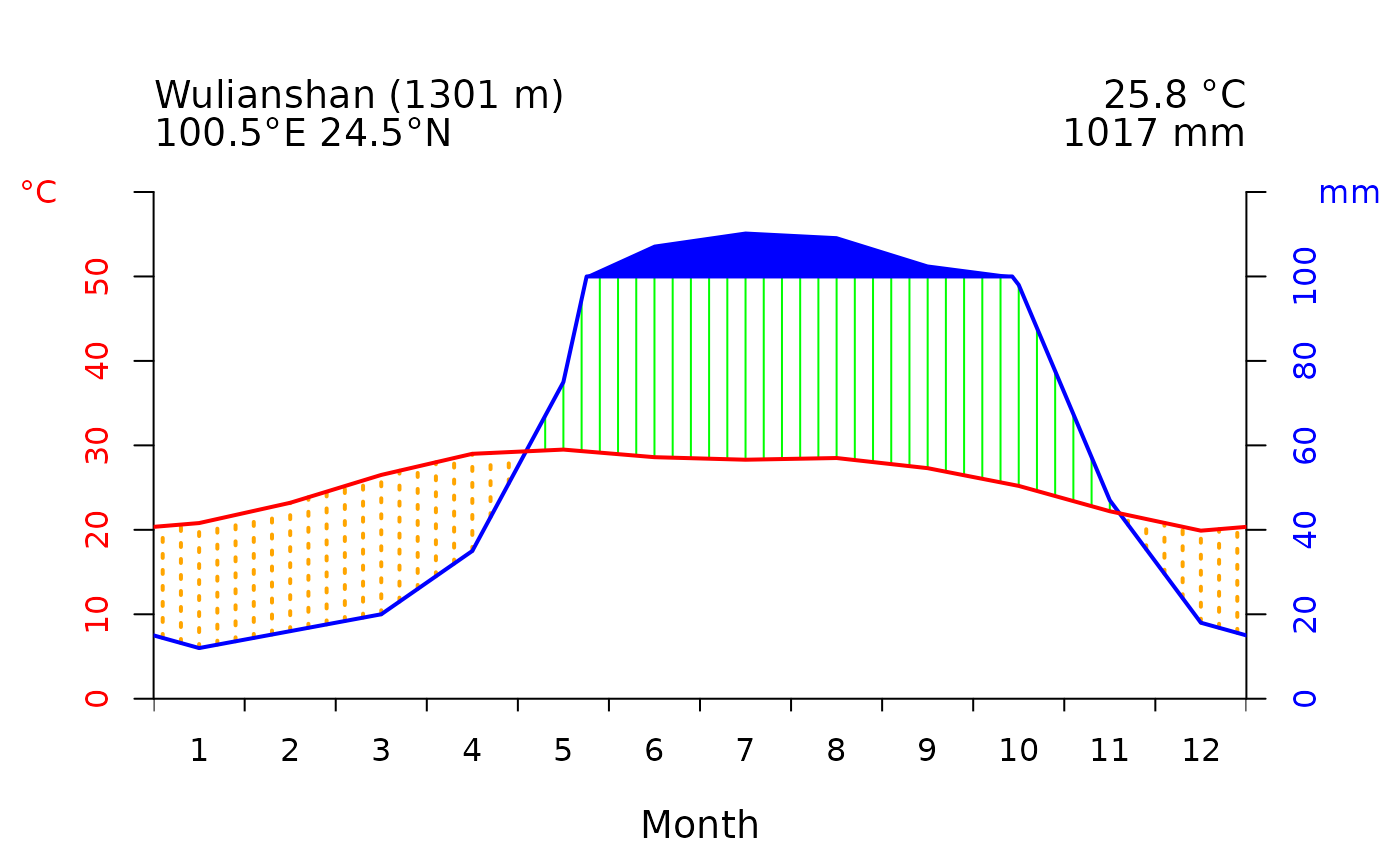
\includegraphics{manual_files/figure-latex/plot1-1.pdf}

在上图中: -
红色曲线代表气温的年际变化,蓝色曲线代表降水的年际变化。这两条曲线闭合形成了两种斑块,表示湿度和干燥程度。竖线填充的斑块代表湿润季节,散点填充的斑块代表干旱季节。与降水曲线颜色相同的多边形表示降水量大于100mm的月份,表示雨季。
-
左上角的信息包括名称、海拔高度和位置坐标。右上方为年平均气温和年平均降水量。

\hypertarget{ux591aux4e2aux5730ux70b9walter-liethux6c14ux5019ux56feux7ed8ux5236ux7684ux89e3ux51b3ux65b9ux6cd5}{%
\subsection{多个地点Walter \&
Lieth气候图绘制的解决方法}\label{ux591aux4e2aux5730ux70b9walter-liethux6c14ux5019ux56feux7ed8ux5236ux7684ux89e3ux51b3ux65b9ux6cd5}}

\texttt{clim\_plot}仅支持一次为一个地点绘制气候图,因为我们建议绘制完成后每张图需要检查,同时向函数导入多个气候数据向量会增加错误的风险。因此,如果您需要自动对多个地点进行绘图,建议使用循环功能:

\begin{Shaded}
\begin{Highlighting}[]
\FunctionTok{data}\NormalTok{(}\StringTok{"plotdata"}\NormalTok{)}
\NormalTok{list }\OtherTok{\textless{}{-}} \FunctionTok{unique}\NormalTok{(plotdata}\SpecialCharTok{$}\NormalTok{No)}
\FunctionTok{par}\NormalTok{(}\AttributeTok{mfrow=}\FunctionTok{c}\NormalTok{(}\DecValTok{1}\NormalTok{,}\DecValTok{1}\NormalTok{))}
\ControlFlowTok{for}\NormalTok{ (i }\ControlFlowTok{in} \DecValTok{1}\SpecialCharTok{:}\DecValTok{5}\NormalTok{)\{}
\NormalTok{ k }\OtherTok{\textless{}{-}}\NormalTok{ list[i]}
\NormalTok{sub }\OtherTok{\textless{}{-}} \FunctionTok{subset}\NormalTok{(plotdata,No}\SpecialCharTok{==}\NormalTok{k)}
\FunctionTok{clim\_plot}\NormalTok{(}\AttributeTok{data=}\NormalTok{sub,}\AttributeTok{ylabel =} \ConstantTok{TRUE}\NormalTok{,}
          \AttributeTok{ylab1=}\StringTok{"Temperature(\textbackslash{}U\{00B0\}C)"}\NormalTok{,}
          \AttributeTok{ylab2=}\StringTok{"Precipitation(mm)"}\NormalTok{,}
           \AttributeTok{p50line =} \ConstantTok{TRUE}\NormalTok{)}
\NormalTok{\}}
\end{Highlighting}
\end{Shaded}

\hypertarget{ux5176ux4ed6ux7ed8ux5236ux6c14ux5019ux56feux7684ux63d0ux793a}{%
\subsection{其他绘制气候图的提示}\label{ux5176ux4ed6ux7ed8ux5236ux6c14ux5019ux56feux7684ux63d0ux793a}}

\hypertarget{ux5728ux6c14ux5019ux56feux4e2dux6807ux8bb0ux971cux51bbux6708ux4efd}{%
\subsubsection{在气候图中标记霜冻月份}\label{ux5728ux6c14ux5019ux56feux4e2dux6807ux8bb0ux971cux51bbux6708ux4efd}}

\begin{Shaded}
\begin{Highlighting}[]
\FunctionTok{data}\NormalTok{(}\StringTok{"plotdata\_Frost"}\NormalTok{)}
\NormalTok{loc }\OtherTok{\textless{}{-}} \FunctionTok{subset}\NormalTok{(plotdata\_Frost,No}\SpecialCharTok{==}\DecValTok{3}\NormalTok{)}
\FunctionTok{clim\_plot}\NormalTok{(}\AttributeTok{data=}\NormalTok{loc,}\AttributeTok{ShowFrost =}\NormalTok{ T)}
\end{Highlighting}
\end{Shaded}

\includegraphics{manual_files/figure-latex/plot frost-1.pdf}

x轴上浅蓝色的方块代表可能出现霜冻的月份,深蓝色表示确定出现霜冻的月份。

\hypertarget{ux6539ux53d8ux989cux8272ux548cux5750ux6807ux8f74}{%
\subsubsection{改变颜色和坐标轴}\label{ux6539ux53d8ux989cux8272ux548cux5750ux6807ux8f74}}

绘图颜色和坐标轴标签可自定义,以满足特定要求。
可以调整温度、降水、湿度、干旱、雨季和霜冻月份块的颜色。

\begin{Shaded}
\begin{Highlighting}[]
\NormalTok{loc }\OtherTok{\textless{}{-}} \FunctionTok{subset}\NormalTok{(plotdata\_Frost,No}\SpecialCharTok{==}\DecValTok{1}\NormalTok{)}
\FunctionTok{clim\_plot}\NormalTok{(loc,}\AttributeTok{pcol =} \StringTok{"\#8DB6CD"}\NormalTok{,}
          \AttributeTok{tcol =} \StringTok{"\#FF6A6A"}\NormalTok{,}
          \AttributeTok{wcol=}\StringTok{"\#4EEE94"}\NormalTok{,}
          \AttributeTok{dcol =} \StringTok{"\#EEB422"}\NormalTok{,}
          \AttributeTok{pfcol=}\StringTok{"\#00BFFF"}\NormalTok{,}
          \AttributeTok{sfcol=}\StringTok{"\#8A2BE2"}\NormalTok{,}
          \AttributeTok{ShowFrost =} \ConstantTok{TRUE}\NormalTok{)}
\end{Highlighting}
\end{Shaded}

\includegraphics{manual_files/figure-latex/color picker-1.pdf}

此外,可以控制轴标签的显示, 并可以使用参数\texttt{ylabel},
\texttt{ylab1}, \texttt{ylab2},
\texttt{mlab}和\texttt{xlab}导入自定义标签。

\begin{Shaded}
\begin{Highlighting}[]
\NormalTok{loc }\OtherTok{\textless{}{-}} \FunctionTok{subset}\NormalTok{(plotdata\_Frost,No}\SpecialCharTok{==}\DecValTok{1}\NormalTok{)}
\FunctionTok{clim\_plot}\NormalTok{(loc,}\AttributeTok{xlab=}\StringTok{"M"}\NormalTok{,}\AttributeTok{mlab =} \StringTok{"en"}\NormalTok{,}
          \AttributeTok{ylabel =} \ConstantTok{TRUE}\NormalTok{,}\AttributeTok{ylab1 =}\StringTok{"Temperature(\textbackslash{}U\{00B0\}C)"}\NormalTok{,}
          \AttributeTok{ylab2 =}\StringTok{"Precipitation(mm)"}\NormalTok{,}\AttributeTok{ShowFrost =} \ConstantTok{TRUE}\NormalTok{)}
\end{Highlighting}
\end{Shaded}

\includegraphics{manual_files/figure-latex/label-1.pdf}

\hypertarget{ux8f85ux52a9ux6807ux8bb0}{%
\subsubsection{辅助标记}\label{ux8f85ux52a9ux6807ux8bb0}}

可选择显示极端温度、降水曲线辅助线、50°C-100mm辅助标记线。

\begin{Shaded}
\begin{Highlighting}[]
\NormalTok{loc }\OtherTok{\textless{}{-}} \FunctionTok{subset}\NormalTok{(plotdata\_Frost,No}\SpecialCharTok{==}\DecValTok{1}\NormalTok{)}
\FunctionTok{clim\_plot}\NormalTok{(loc,}\AttributeTok{p3line =} \ConstantTok{TRUE}\NormalTok{,}
          \AttributeTok{p50line =} \ConstantTok{TRUE}\NormalTok{,}
          \AttributeTok{extremeT =} \ConstantTok{TRUE}\NormalTok{,}\AttributeTok{ShowFrost =} \ConstantTok{TRUE}\NormalTok{)}
\end{Highlighting}
\end{Shaded}

\includegraphics{manual_files/figure-latex/auxiliary line-1.pdf}

\hypertarget{ux53c2ux8003ux6587ux732e}{%
\section{参考文献}\label{ux53c2ux8003ux6587ux732e}}

\begin{enumerate}
\def\labelenumi{\arabic{enumi}.}
\item
  Guijarro J A (2023). climatol: Climate Tools (Series Homogenization
  and Derived Products), 4.0.0.,
  \url{https://CRAN.R-project.org/package=climatol}.
\item
  Fick, S.E. and R.J. Hijmans, (2017). WorldClim 2: new 1km spatial
  resolution climate surfaces for global land areas. International
  Journal of Climatology 37 (12): 4302-4315.
\item
  Harris, I., Osborn, T.J., Jones, P.D., Lister, D.H. (2020). Version 4
  of the CRU TS monthly high-resolution gridded multivariate climate
  dataset. Scientific Data 7: 109.
\item
  Walter H \& Lieth H (1960): Klimadiagramm Weltatlas. G. Fischer, Jena.
\end{enumerate}

\end{document}
